
\begin{figure}[!htb]
    \centering
    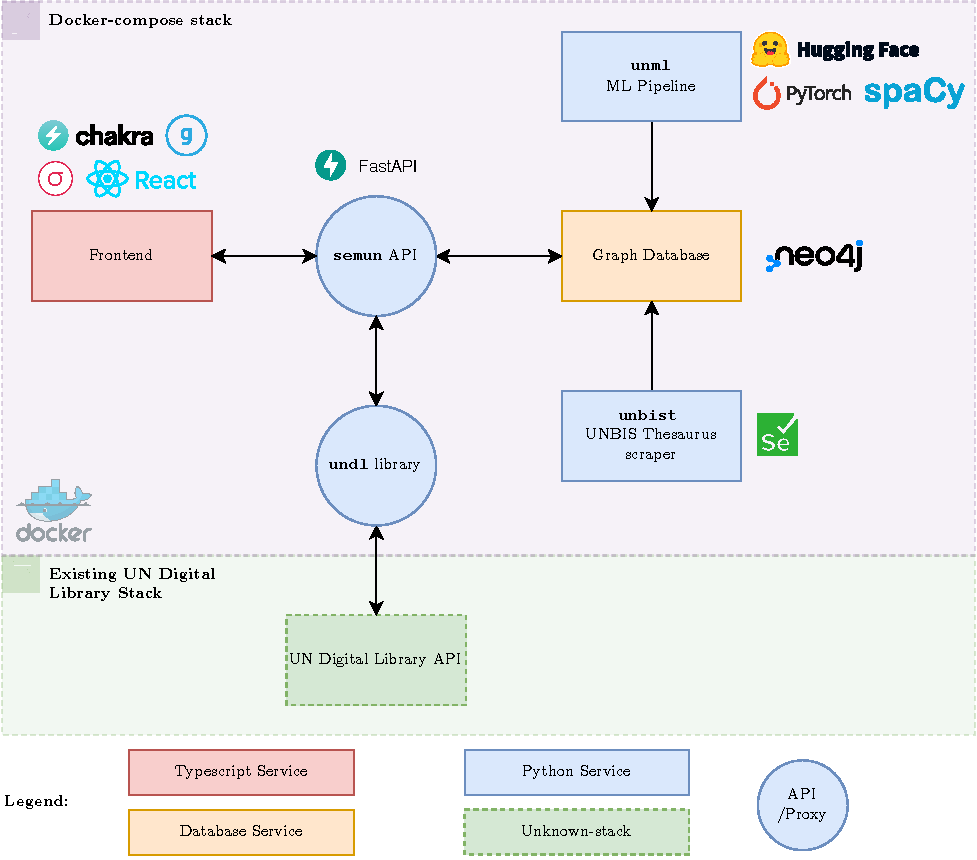
\includegraphics[width=\textwidth]{res/architecture-final.pdf}
    % \includegraphics*[width=0.8\textwidth]{res/architecture-final.png}
    \caption{Final stack architecture}
    % change caption position to the bottom

    \label{fig:architecture}
\end{figure}

\section{Final architecture} \label{sec:final-architecture}

The final architecture is a full-stack architecture, from the database to the frontend, handed in as a Docker compose stack: \href{https://github.com/ClementSicard/un-semun}{\faGithub{} \texttt{un-semun}}.

The project consists of $7$ \faGithub{} GitHub repos:

\begin{itemize}
    \item \href{https://github.com/ClementSicard/un-semun}{\faGithub{} \texttt{un-semun}}: The main repository with the \texttt{docker-compose} stack declaration.
    \item \href{https://github.com/ClementSicard/un-semun-frontend}{\faGithub{} \texttt{un-semun-frontend}}: The frontend.
    \item \href{https://github.com/ClementSicard/un-semun-api}{\faGithub{} \texttt{un-semun-api}}: The API for the frontend.
    \item \href{https://github.com/ClementSicard/undl}{\faGithub{} \texttt{undl}}: The code for \texttt{undl}, a Python wrapper around the UN Digital Library API.
    \item \href{https://github.com/ClementSicard/un-unbis-thesaurus-scraper}{\faGithub{} \texttt{un-unbis-thesaurus-scraper}}: A scraper for the UNBIS Thesaurus taxonomy website.
    \item \href{https://github.com/ClementSicard/un-ml-pipeline}{\faGithub{} \texttt{un-ml-pipeline}}: Machine learning pipeline for UNDL documents.
    \item \href{https://github.com/ClementSicard/un-semun-misc}{\faGithub{} \texttt{un-semun-misc}}: Diverse scripts used for the project.
    \item \href{https://github.com/ClementSicard/un-semun-paper}{\faGithub{} \texttt{un-semun-paper}}: The code for this paper.
\end{itemize}

This paper will go through each of them in detail except for the paper repository.



\subsection{\texttt{un-semun-frontend}: A React \& Sigma.js frontend} \label{ssec:un-semun-frontend-a-react-sigma-js-frontend}

I used React combined with Typescript for the UI framework, as well as \href{https://chakra-ui.com/}{Chakra UI} for the UI components and \href{https://www.sigmajs.org/}{\texttt{Sigma.js}} via its React adapter \href{https://sim51.github.io/react-sigma/}{\texttt{@react-sigma}} for the network map. \href{https://graphology.github.io/}{\texttt{graphology}} was also used for graph manipulation in the frontend, mostly to iterate over graph elements to perform styling. The code is available here: \repo{un-semun-frontend}.



\todo[inline]{Add an actual screenshot of the frontend}

\begin{figure}[!htb]
    \centering

    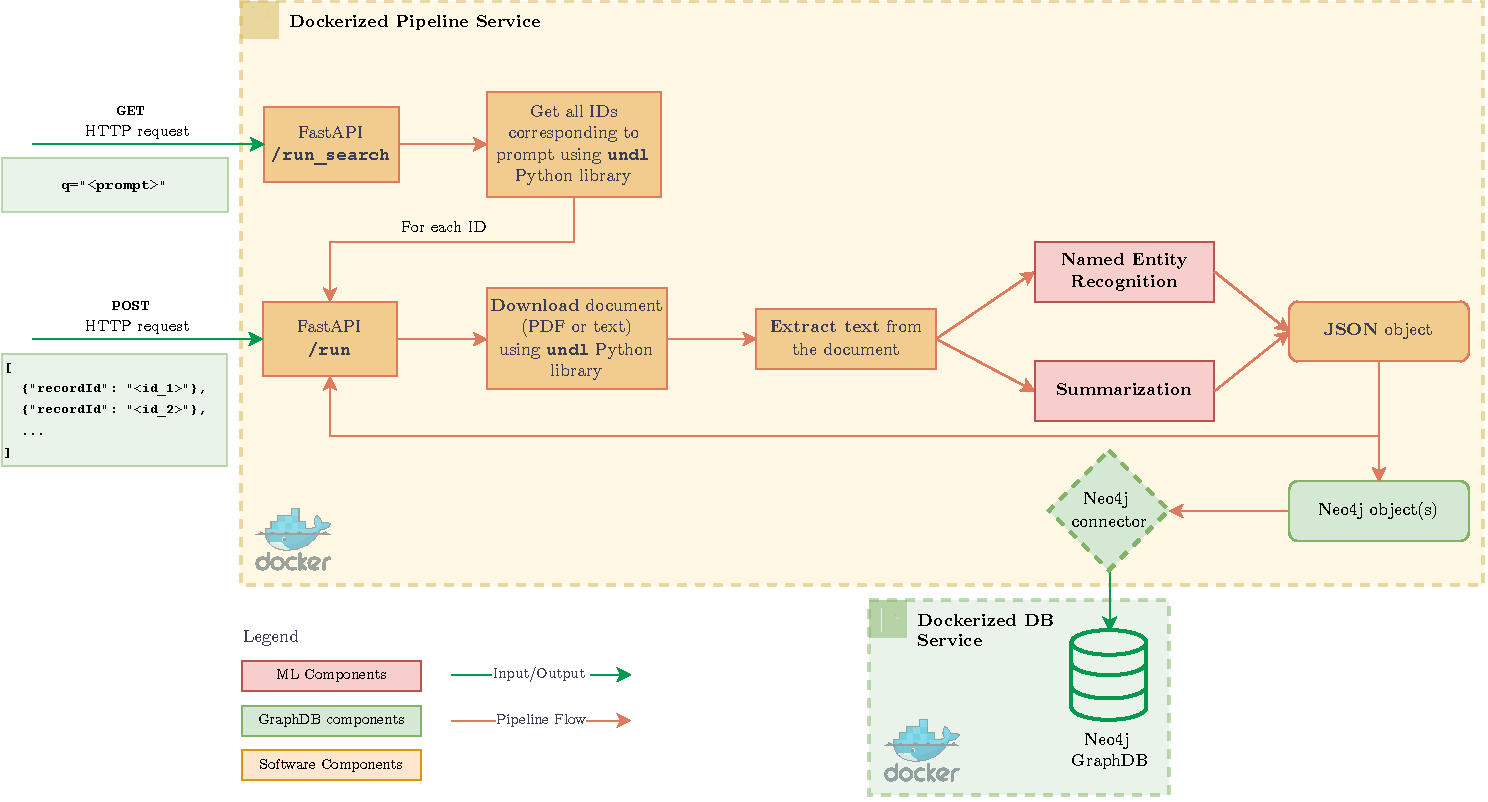
\includegraphics[width=\textwidth]{res/ml-pipeline.pdf}
    \caption{\texttt{un-semun-frontend} library: a dockerized machine learning pipeline for NER \& summarization}
    % change caption position to the bottom

    \label{fig:frontend-screenshot}
\end{figure}


The frontend was the part I was the least familiar with, but Chakra UI allowed to insert nice-looking components that I could customize based on my use case. It is composed in two panes:

\begin{itemize}
    \item \textbf{The search bar} (on top): the user can enter its prompt, which will be sent to the API (\ref{ssec:un-semun-api-an-api-for-un-semun-frontend-using-fastapi}) to retrieve the results.
    \item \textbf{The result list} (on the left). The results are displayed as a scrollable list of \texttt{Card} components, with the title, the summary, and the date of publication. The user can click on a card to display the document in the right pane.
    \item \textbf{The network map} (on the right). The results of the search are also displayed as a network map, with the documents, related United Nations bodies, topics from UNBIS Thesaurus taxonomy, and named entities extracted from the documents. The user can click on a node to display the document in the left pane. This map is also fetched using the API (\ref{ssec:un-semun-api-an-api-for-un-semun-frontend-using-fastapi}) and is based on the results of the machine learning pipeline (\ref{ssec:un-ml-pipeline-the-machine-learning-pipeline}).
\end{itemize}




\subsection{\texttt{un-semun-api}: An API for \texttt{un-semun-frontend} using \texttt{FastAPI}} \label{ssec:un-semun-api-an-api-for-un-semun-frontend-using-fastapi}

The \texttt{un-semun-api} Python package was developed to provide an API for the frontend. It is a \href{https://fastapi.tiangolo.com/}{\texttt{FastAPI}} application, which is a Python framework for building APIs. It is a modern framework, which is fast, easy to use, and well documented. One nice feature is that it is also coupled with \href{https://docs.pydantic.dev/latest/}{\texttt{pydantic}} to perform data validation and serialization. This is very useful to ensure that the data sent to the frontend is valid, and to avoid having to write boilerplate code for serialization and deserialization.

This package mainly acts as a proxy between the frontend and the UNDL API, and is composed of $2$ main endpoints:

\begin{itemize}
    \item \texttt{/search}: This endpoint is used to perform a search query.  It takes a \texttt{GET} HTTP request with query parameter the prompt. Then, it uses \texttt{undl} (\ref{ssec:undl-a-python-library-to-wrap-to-the-un-digital-library-api}) library to perform the search on the UNDL API and returns the results to the frontend.
    \item \texttt{/graph}: This endpoint is used to get the graph corresponding to the above search query, also with an HTTP \texttt{GET} request with the prompt as unique query parameter. To optimize the process, it first gets the IDs of all documents returned by the search query on the given prompt, then it queries the Neo4j graph database (\ref{ssec:neo4j-graph-database}) to get the graph corresponding to these documents. Finally, it returns the graph to the frontend as \texttt{JSON} structured according to the format expected by the \href{https://graphology.github.io/}{\texttt{graphology}} Typescript library, which is used to model a graph and manipulate it as a programmatic object.
\end{itemize}

Note that the API is dockerized and that it offers a basic query caching mechanism to avoid querying the UNDL API too often. This is done using a simple \texttt{dict} in memory, which is not ideal but enough for the scope of this project.


\subsection{\texttt{undl}: A Python library to wrap to the UN Digital Library API} \label{ssec:undl-a-python-library-to-wrap-to-the-un-digital-library-api}

\subsubsection*{Tech stack of \texttt{undl}} \label{sssec:tech-stack-of-undl}

For the \texttt{undl} library, I used Python 3.10 with packages, with \texttt{requests} for the HTTP requests, \texttt{pandas} for the data manipulation, and \texttt{pydantic} for the data validation.


\todo[inline]{Intermediary between frontend and Neo4j}
\todo[inline]{Proxying the UNDL API using \texttt{undl} library}



% UNBIST
\subsection{\texttt{un-unbis-thesaurus-scraper}: the UNBIS Thesaurus scraper} \label{ssec:un-unbis-thesaurus-scraper-the-unbis-thesaurus-scraper}

\repo{un-unbis-thesaurus-scraper} is a Python scraper that crawls the UNBIS Thesaurus website\footnote{\url{https://research.un.org/en/thesaurus}} and extracts the thesaurus terms and their relations. Once all the Thesaurus entries have been parsed, they are inserted with all their fields to the graph database instance (\ref{ssec:neo4j-graph-database}).

It is mainly used to link Thesaurus topics the documents which are passed through the machine learning pipeline (\ref{ssec:un-ml-pipeline-the-machine-learning-pipeline}), but I felt it was also interesting to be able to visualize all the topics together and how they're related, so I built and deployed a small Vercel app to do so: \href{https://un-graph-ui.vercel.app/}{\faCloud{} \texttt{https://un-graph-ui.vercel.app/}}, which is built on a similar stack as the frontend (\ref{ssec:un-semun-frontend-a-react-sigma-js-frontend}).



% unml
\subsection{\texttt{un-ml-pipeline}: The machine learning pipeline} \label{ssec:un-ml-pipeline-the-machine-learning-pipeline}

\repo{un-ml-pipeline} is the main component of this project. It englobes a Python library, \texttt{unml}, as well as an API wrapping it. It functions as follows (see Figure \ref{fig:ml-pipeline}):
\todo[inline]{Connection to Neo4j}


\begin{figure}[!htb]
    \centering

    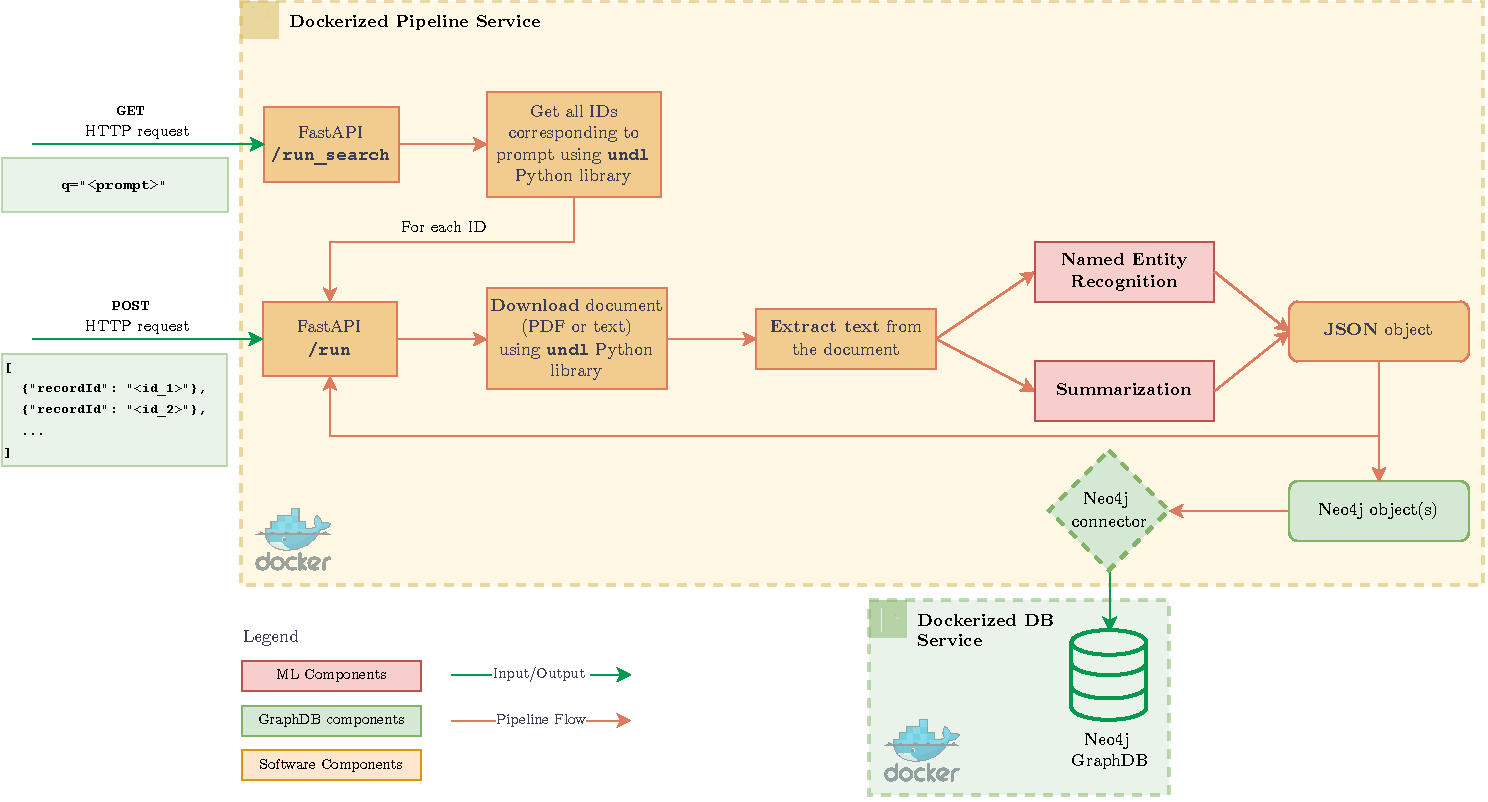
\includegraphics[width=\linewidth]{res/ml-pipeline.pdf}
    \caption{\texttt{unml} library: a dockerized machine learning pipeline for NER \& summarization}
    % change caption position to the bottom

    \label{fig:ml-pipeline}
\end{figure}

The pipeline API is a \texttt{FastAPI} app, which exposes two endpoints. The \texttt{run} endpoint gets an ID as input, and works as follows:

\begin{enumerate}
    \item A client sends an HTTP \texttt{POST} request to the pipeline API on \texttt{run} endpoint, with the payload containing a list of JSON objects with a \texttt{recordId}. (Note: this is arguably not an optimal data structure to store the IDs, but it was the easiest way to make \texttt{pydantic} happy and validate the input data structure.)

    \item Use \texttt{undl}'s client \texttt{queryBdId} method to download the corresponding document complete information and PDF document. Sometimes it doesn't exist – if it is the case, create a JSON with solely the information from the UNDL API, and jump to step $6$

    \item Extract the text from the PDF document using \texttt{PyMuPDF}\footnote{\url{https://github.com/pymupdf/PyMuPDF}} library.

    \item Then the pipeline is split into $2$ parts:
          \begin{itemize}
              \item \textbf{Named Entity Recognition}: Extract named entities from the document. All types entities are collected (the types can vary depending on the model used though), but for data quality reasons, only UN bodies and Countries are actually stored in the graph database and linked to the document. However, the other entities are still returned by the API at the end of a pipeline run, and can be used for further analysis.

              \item \textbf{Summarization}: The document is being summarized using a deep learning model, and the chosen model is a parameter of the pipeline (see Table \ref{tab:summarization-models} for more details). The summary for a document is then stored in the database to enhance the nodes.
          \end{itemize}
    \item The results of the machine learning components (e.g., the summary and the extracted named entities) are then stored into a JSON object
    \item The JSON object is converted to a Cypher (the graph database, Neo4j, query language) query and then the query is run against the Neo4j database to update the graph. Note that the Neo4j instance lives in another Docker container to better compartmentalize the stack.
\end{enumerate}


The machine learning pipeline also offers the \texttt{run\_search} endpoint, which receives a prompt as input (e.g., \texttt{"Peacekeeping"}), and works as follows:

\begin{enumerate}
    \item A client sends an HTTP \texttt{GET} request to the pipeline API on \texttt{run\_search} endpoint, with the prompt as a query parameter \texttt{q}.
    \item The pipeline API queries UNDL API against the given prompt and collects document IDs corresponding to the search results using \texttt{getAllRecordIds} method from \texttt{undl}'s. It then returns the list of IDs.
    \item For each record ID, do what querying \texttt{run} endpoint does
\end{enumerate}

\subsubsection{Models} \label{sssec:models}

When it came to choosing a model for both tasks, the main criteria were the following:
\begin{itemize}
    \item The model needs to be accurate
    \item The model needs to have fast inference due to the large number of documents the pipeline could have to deal with.
    \item The model should ideally have optimized inference for CPU, as the pipeline would preferably not be GPU-accelerated for cost reasons.
\end{itemize}

Hence, I decided to use the \texttt{transformers} library by HuggingFace, coupled with their SafeTensors\footnote{\url{https://huggingface.co/docs/safetensors/index}} technology for faster loading and \texttt{accelerate}\footnote{\url{https://huggingface.co/docs/accelerate/index}} Python library for faster inference on CPU. Some models also offered ONNX runtime binaries, but not all of them, so I didn't bother using them – this might however be a good idea for future work and to keep this pipeline cost-efficient.

For summarization, one of big challenges when choosing a model was that it should handle a very number of tokens as input. Indeed, the self-attention layer in the transformer architecture scales quadratically with the input length. Hence, transformers are often non-suited for very large inputs – and reports from the UNDL are sometimes very long and counts $100$k+ tokens. I came up with these two solutions to address this issue:

\begin{itemize}
    \item \textbf{Divide \& Conquer approach}: Recursively split and summarize the document into smaller chunks, then concatenate the summaries and pass them into the model until the length of the result summary is below fixed threshold.

    \item \textbf{Use transformers models that offer a very large input size}: Some models like LongT5 or LongFormer replace the self-attention mechanism with a custom attention mechanism that scales linearly with the input. This allows them to handle very large inputs. However, they are not as accurate as the other models, and they are also slower to train and to run inference on.
\end{itemize}

Here is a comparison of the models I used for the summarization task:

\begin{table}[!ht]
    \centering
    \small
    \begin{tabular}{p{2cm}p{2.5cm} p{2.5cm} p{2.5cm} p{2.5cm} p{2cm}}
        \toprule
                                      & \textbf{DistilBART-CNN}                                     & \textbf{DistillBART-XSUM}                                    & \textbf{DistilPegasus-CNN}                                       & \textbf{LongFormer} (\textit{default})                       & \textbf{LongT5}                                                                \\
        \midrule
        \textbf{File}                 & \github{unml/models/summarize/DistilBARTCNN.py}             & \github{unml/models/summarize/DistilBARTXSUM.py}             & \github{unml/models/summarize/DistilPegasusCNN.py}               & \github{unml/models/summarize/LED.py}                        & \github{unml/models/summarize/LongT5.py}                                       \\
        \textbf{Paper}                & \extlink{https://arxiv.org/pdf/2010.13002.pdf}{arXiv}       & \extlink{https://arxiv.org/pdf/2010.13002.pdf}{arXiv}        & \extlink{https://arxiv.org/pdf/2010.13002.pdf}{arXiv}            & \extlink{https://arxiv.org/pdf/2004.05150}{arXiv}            & \extlink{https://arxiv.org/pdf/2112.07916}{arXiv}                              \\
        \textbf{Authors}              & Shleifer et al.                                             & Shleifer et al.                                              & Shleifer et al.                                                  & Beltagy et al.                                               & Guo et al.                                                                     \\
        \textbf{Company}              & HuggingFace                                                 & HuggingFace                                                  & Google                                                           & Allen AI                                                     & Google                                                                         \\
        \textbf{Year}                 & 2020                                                        & 2020                                                         & 2020                                                             & 2020                                                         & 2022                                                                           \\
        \textbf{HuggingFace Model}    & \link{https://huggingface.co/sshleifer/distilbart-cnn-12-6} & \link{https://huggingface.co/sshleifer/distilbart-xsum-12-1} & \link{https://huggingface.co/sshleifer/distill-pegasus-cnn-16-4} & \link{https://huggingface.co/pszemraj/led-base-book-summary} & \link{https://huggingface.co/pszemraj/long-t5-tglobal-base-16384-book-summary} \\
        \textbf{Max Token Input Size} & $1'024$                                                     & $1'024$                                                      & $1'024$                                                          & $16'384$                                                     & $16'384$                                                                       \\
        \textbf{Params}               & 306M                                                        & 222M                                                         & 370M                                                             & 162M                                                         & 248M                                                                           \\
        \bottomrule
    \end{tabular}
    \caption{Models used for summarization task}
    \label{tab:summarization-models}
\end{table}



For Named Entity Recognition (NER) tasks, other models than FLERT work slightly better but are much slower due to their much larger number of parameters. In addition, spaCy has optimized inference for CPU, which is a big plus for this project. Here is a comparison of the models I used for the NER task:

\begin{table}[ht]
    \centering
    \small
    \begin{tabular}{p{4cm}p{3.2cm} p{2.5cm} p{4cm}}
        \toprule
                                   & \textbf{FLERT} (\textit{default S})                  & \textbf{RoBERTa}                                                      & \textbf{spaCy  \texttt{en\_core\_web\_trf}}         \\
        \midrule
        \textbf{File}              & \github{unml/models/ner/FLERT.py}                    & \github{unml/models/ner/RoBERTa.py}                                   & \github{unml/models/summarize/DistilPegasusCNN.py}  \\
        \textbf{Paper}             & \extlink{https://arxiv.org/abs/2011.06993}{arXiv}    & \extlink{https://arxiv.org/abs/1907.11692}{arXiv}                     & -                                                   \\
        \textbf{Authors}           & Akbik et al.                                         & Liu et al.                                                            & -                                                   \\
        \textbf{Company}           & Flair NLP                                            & Meta (fine-tune HuggingFace)                                          & spaCy                                               \\
        \textbf{Year}              & 2020                                                 & 2019                                                                  & 2023 (\texttt{v3.6.1})                              \\
        \textbf{HuggingFace Model} & \link{https://huggingface.co/flair/ner-english-fast} & \link{https://huggingface.co/Jean-Baptiste/roberta-large-ner-english} & \link{https://huggingface.co/spacy/en_core_web_trf} \\
        \textbf{Params}            & {20M(S) 560M(L)}                                     & 355M                                                                  & 355M                                                \\
        \bottomrule
    \end{tabular}
    \caption{Models used for NER task}
    \label{tab:ner-models}
\end{table}

\pagebreak
\subsection{Neo4j graph database} \label{ssec:neo4j-graph-database}

A graph database seemed to be the best choice to store the data extracted from the documents and the links between them, since it captures this relationship property and is able to retrieve it very efficiently. \href{https://neo4j.com/}{\texttt{Neo4j}} seemed to be the most accessible one to use, but other solutions exist (such as ArangoDB\footnote{\url{https://www.arangodb.com/}} or OrientDB\footnote{\url{https://orientdb.org/}}).

Here is the chosen data model for this project:

\subsubsection{Types of nodes} \label{sssec:types-of-nodes}

\begin{itemize}
      \item \texttt{Document}:
            This node type represents a document in the UNDL. It contains the document's \texttt{id} from the library management system, its summary (created when the document was run through the machine learning pipeline), symbol (some internal UN classification for the document - for instance \texttt{A/C.5/43/SR.50}), publication date, title, URL, and publication location.

      \item \texttt{Topic}:
            This node type represents a topic in the sense of the UNBIS Thesaurus taxonomy. I made a scraper \repo{un-unbis-thesaurus-scraper} (\ref{ssec:un-unbis-thesaurus-scraper-the-unbis-thesaurus-scraper}), and used it to retrieve all the topics from the taxonomy website, and inserted them into the database instance. Each topic has \texttt{name}, \texttt{cluster}, \texttt{id} fields, as well as label fields for each of the $6$ official UN languages (\texttt{labelEn}, \texttt{labelFr}, \texttt{labelEs}, \texttt{labelAr}, \texttt{labelZh}, \texttt{labelRu}).

      \item \texttt{MetaTopic}:
            UNBIS Thesaurus is structured as a hierarchy, and a \texttt{MetaTopic} is one of the top-level topics in this hierarchy. It has the same fields as a \texttt{Topic} node, and there are $18$ of them.\footnote{\href{https://metadata.un.org/thesaurus/?lang=en}{The list of \texttt{MetaTopic} nodes from UNBIS Thesaurus website}}

      \item \texttt{Country}:
            This node type represents a country as a member state of the UN. It has the same fields as a \texttt{Topic} node, and there are $193$ of them.\footnote{\href{https://www.un.org/en/about-us/member-states}{The list of the $193$ UN member states from the UN website}} The data to create these nodes was retrieved from the UN website, and the Cypher queries were generated using a Python script in \repo{un-semun-misc} (\ref{ssec:un-semun-misc}).

      \item \texttt{UNBody}:
            This node type represents a body of the United Nations. A body of the UN is an organizational unit within the United Nations system, established to carry out specific functions ranging from peacekeeping and humanitarian aid to diplomatic negotiations and policy recommendations. Some famous examples include the Security Council, the World Health Organization (WHO), the International Monetary Fund (IMF) etc... As for the countries, the data was retrieved from the UN website, and the Cypher queries were generated using a Python script in \repo{un-semun-misc} (\ref{ssec:un-semun-misc}).


\end{itemize}

\subsubsection{Types of relationships} \label{sssec:types-of-relationships}

These nodes are linked together by the following relationships:

\begin{itemize}
      \item \texttt{-[REFERENCES]->}:
            This relationship type links a \texttt{Document} node to a \texttt{Country} or \texttt{Entity} node, and is self-explanatory: the document references the target entity. This relationship is extracted by the machine learning pipeline.

      \item \texttt{-[HAS\_SUBTOPIC]->}:
            Links a \texttt{MetaTopic} node to a \texttt{Topic} node to explicit the hierarchy between the two nodes. It was created by the scraper.

      \item \texttt{-[IS\_ABOUT]->}:
            Links a \texttt{Document} node to a \texttt{Topic} node to indicate that the \texttt{Document} has been classified by UN Digital Library staff as a document about the \texttt{Topic}. This relationship is extracted from the UNDL API response.

      \item \texttt{-[RELATED\_TO]->}:
            Links a \texttt{Topic} node to another \texttt{Topic} node indicate a semantic link between the two topics. This relationship is extracted from the UNBIS Thesaurus website, using the scraper as well.

\end{itemize}



\subsection{\texttt{un-semun}: The main repository} \label{ssec:un-semun-the-main-repository}

\texttt{un-semun} is a repository that englobes all other repositories as submodules. It also contains the \texttt{docker-compose} stack declaration, which points to Dockerfiles in submodules. They are updated using the \texttt{Makefile} when new commits are added to the submodules. The port forwardings and environment variables are also declared here. This is the main entry point to run the whole stack.




\subsection{\texttt{un-semun-misc}} \label{ssec:un-semun-misc}







\subsection{General tech stack notes} \label{ssec:general-tech-stack-notes}

For all the Python components, the dependencies are managed using \href{https://github.com/python-poetry/poetry}{\texttt{poetry}}. They are also all dockerized, and the whole stack is orchestrated using \href{https://docs.docker.com/compose/}{\texttt{docker-compose}}.
